\documentclass[10pt,a4paper]{article}
\usepackage[top=1in, left=1in, right=1in, bottom=1.5in]{geometry}
\usepackage{titlesec}
\usepackage{graphicx}

% Custom LaTeX macros used throughout the document
% Code font
\newcommand{\cf}{\ttfamily}


\begin{document}
\begin{center}
  {\huge\bfseries Github Issue Tracker Searcher\par}
  \vspace{1cm}
  {\Large\itshape Andrew Lewis, Francisco Santana, Todd Gaunt\par}
  \vspace{0.5cm}
  {\large\today\par}
\end{center}

\section{Introduction}

Issue trackers are a commonly used tool along side version control systems such
as git or svn. The tools allow for users or developers to submit a feature
request, bug fix, or even just a question and have it be responded to, resolved,
and even linked to a specific patch that was made to fix a bug. To improve upon
such a system, letting a developer know what files he is likely to need to change
based on the text-body of an issue may help expedite the process of feature
implementation or bug fixing. This turns the task of the developer to think about
exactly where in the code-base he must update, a task of remembering project
layout in his head, into a yes/no problem when given a list of suggested files
to edit; Able to see at a glance and reaffirm with himself which files he should
be working in.

Programming projects on Github are able to use the websites pull request and
issue tracking system, and it is a well-featured issue-tracker at that. Since
github has many users, and many projects that utilize its issue tracker, GHITS
was developed to take advantage of this to provide a file searcher for
issue tracking described here.

\section{Related Work}

There is no specific work we refer to, other than the Information Retrieval methods we learned in the CS 753 class. The query expansion methods that are described later were graciously provided by Professor Dietz, and also involved some custom work in the case of the coinflip model

\section{Approach}

The methods we implemented are TF-IDF variants, language models, and query expansion models. A method for future implementation is a feature-based ranking model using TF-IDF and LM as features and using training data to find the best weighting. The two models of query expansion were a random “coinflip” method to translate from the query language to the source language, and a thesaurus extraction method.
  
Term frequency-inverse document frequency (TF-IDF) is a standard information retrieval method that tries to solve some of the issues that arise when indexing files. Its use is to adjust the weighting of terms according to intuitions about the rarity of a term and the document length. The implementation of TF-IDF in Lucene requires creating a new instance of TFIDFSimilarity, overriding its functions to fit the desired variation, then passing it to the IndexSearcher. In our system, three variations are implemented: lnt.ltn, ann.apn, and bnn.bnn.

In attempt to solve the gap between natural language and code, a global query expansion method was chosen. This method is called automatic thesaurus generation. The main idea is to index a training set of data into a term-document matrix, and find the co-occurrences between all the terms. To do this, the term-document matrix is multiplied with the transpose of itself, resulting in a matrix of similarity weights that correspond between every term in the training set. Using these similarity scores, a thesaurus (mappings) is built containing all the terms and the synonyms they co-occur with. 

    $A = term-document matrix$
    $C = A*AT = co-occurrence matrix$

In the context of our task definition, this thesaurus generation was done slightly differently. We treated a Document as a single issue-code pairing from the training set. The first term-document matrix AI is built by issue terms -> issue-code documents, and the second term-document matrix AC is built by code terms -> issue-code documents. Applying ltc tf-idf weighting to both the matrices, then performing AI*ACT gave us the co-occurrence matrix C of issue terms to code terms. A threshold of 0.05 or a max of three synonyms was used to create the mappings.

The other algorithm for query expansion implemented was a random translation model named
"coin flip". The method was actually conceived as a placeholder / baseline method that was supposed
to be used to compare more intricate methods that try to be smart about how they
expand a query. The coin flip model is a method that generates a word mapping
from query language to corpus language via training data, and requires it to function
effectively.

Essentially, for every query in the training set there is a set of files
associated with the query that are considered relevant, given in this case the
pull request diff file. These are the files that would ideally be returned given
a perfect search model. The coinflip model then takes every word in the training
query, however it may be tokenized, and then inserts that word into a string to
string mapped dictionary of words. The key in this dictionary is the query term
itself, and the value associated with each query term is randomly chosen from the
set of relevant documents given by the pull request diff file at random. Yes, at
random.

The file generated by the coinflip method is a json representation of this mapping.
Each word in the query language (which is all tokens encountered in the training set)
are mapping one-to-one with words from the corpus. This was not expected to perform
well because of its random nature which would not seem to produce any
actual meaningful translation mapping. Bias is introduced towards certain words
in the training set using this method, however, because it only maps query terms
to document terms appearing in relevant files. This hypothetically should bias
the randomly assigned word to create better search results, since not all terms
appear in all documents at the same frequency or at all.

\section{Evaluation}

Our data set consists of Github pull requests from the “Sway Window manager” Github repo. A Python script was made to make calls to the Github API to scrape the title+description and file diff list from 1000 Github issues. This data was split into a training set and a testing set, serving as our ground truth for training and evaluation. The corpus that was indexed was the source code from the “Sway window manager” Github repository found here: https://github.com/swaywm/sway. Given a query—that is, text representing a Github issue—GHITS performs a search on the indexed corpus and returns a ranked list of relevant files.

We compare Lucene’s default BM25, TF-IDF variant lnc.ltn, laplace smoothing, and our query expansion methods using MAP, NDCG, and Precision@R as our evaluation measures. The results are shown below in the graph and table. 

The methods did not achieve the results we expected, and overall underperformed such that the tool itself may not be helpful. An important note to be made is that our system only indexed four file types, when groud truth we evaulated against contained other filetypes. The results are, however, quite good compared to just returning random results. There were some notable differences between some of the methods, specifically the query expansion methods. The best method was the “coinflip” algorithm that utilized random assignment during the thesaurus building. The baseline method, BM25 (Lucene’s default) performed okay for each metric for an untuned search method. Unfortunately, the global thesaurus generation method performed the worse than expected, worse than BM25 on all metrics.

The challenge to bridge the gap between English plain text and code explains the generally low scores. Using the global thesaurus generation made sense intuitively, but came with its own difficulties: how the source code files are to be tokenized, and how is the threshold set for selected synonyms of a issue term. The use of custom analyzers for different files types may alleviate much of the tokenizing issues, and maybe the use of bigrams or trigrams with issue and/or code terms could be a potential improvement. Finding a more accurate way of selecting synonyms from the co-occurrence matrix, and filtering known false synonyms would also be an improvement. The downside to query expansion though is that it introduces many false positives due to altering the initial query, which could quite plainly just be injecting noise/junk into the semantics of the query.

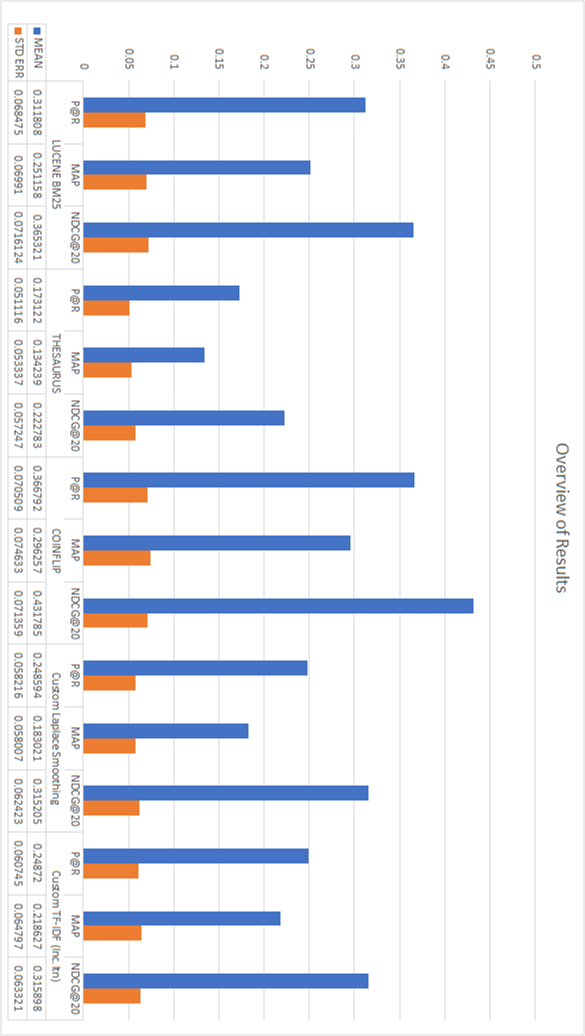
\includegraphics[height=10in]{graph.png}

A possible reason to explain the coin flip model’s performance could be that by assigning a random word from a small selection relevant docs per query term, rather than the entire corpus, that there is a decent chance that a long and infrequent term inside the document is being assigned to a unique query term that most commonly appears in queries that relate to a specific set of files. This could be worth investigating to see if it is indeed sufficient to find unique terms amongst each set and map them together with the hopes that they are related based on the training data provided.


\section{Conclusion and Future Work}

The best model found for query expansion was the custom "coin flip" method described in
this paper, although they all ranked lower than desired on all metrics due to the difficulty
in translating plain english to code without looking at semantics or intent of the text.

For future project expansions on this work, it would be nice to see learning to
rank with TF-IDF and LM models and see how it can be improved with the Thesaurus
and coin flip method.

Coin flip can also be modified to bias the translation assignment to favor
long, unique words in the translation mapping between the query language and the
document language, rather than just completely at random. This way, whenever
certain keywords appear in a query, they are likely mapped to terms that appear
in only a few specific files. This is postulated to improve the results of coin
flip drastically since it is an unbiased random assignment currently. Along
these same lines, small words or words that are frequent across all documents
such as "was", "fix", "change", etc... could be left out of the translation
since they would not be good indicatators of relevancy, since certain terms can
appear in any pull request and thus have no meaning.

\section{Contributions}

Andrew: Thesaurus extraction method
Todd: Github issue web scraper, CoinFlip probabilistic query expansion method
Francisco: Evaluation tool, custom TF-IDF and LM feature classes

\end{document}
